\documentclass{article}
\usepackage[T1]{fontenc}
\usepackage[latin2]{inputenc}
\usepackage[english]{babel}
\usepackage{tikz}
\usepackage{times}
\usetikzlibrary{calc,through,backgrounds,positioning,fit}
\usetikzlibrary{shapes,arrows,shadows}
 
\begin{document}
 
 
\centering
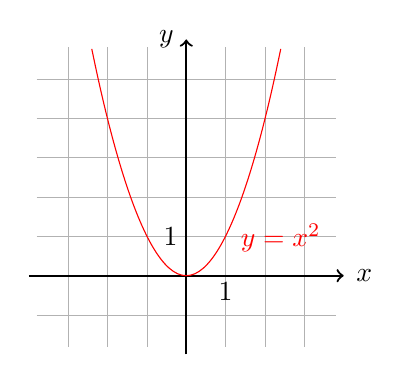
\begin{tikzpicture}[scale=1,inner sep=0.4mm]
\draw[step=5mm,draw=black!30!white,very thin] (-1.9,-0.9) grid (1.9,2.9);
\draw[thick] [->] (-2,0) -- (2,0) node [right=3pt] {$x$};
\draw[thick] [->] (0,-1) -- (0,3) node [left=3pt] {$y$};

\draw [red] (0,0) parabola (1.2, 2.88);
\draw [red] (0,0) parabola (-1.2, 2.88);

\node (p1) at (0.5,-0.2)  {$1$};
\node (p2) at (-0.2,0.5)  {$1$};
\node [red] (t) at (1.2,0.48)  {$y=x^2$};
\end{tikzpicture}
 
\end{document}